\section{Discusión}

\subsection{Traceroute a Universidades}

A continuación mostramos diferentes traceroutes a universidades en diferentes continentes. Consideramos que esto es relevante dado que nos permitirá observar enlaces intercontinentales y otras particularidades. El RTT promedio se calculo a partir de 5 requests, tomando como tiempo inicial y final el tiempo dado por los paquetes IP. No utilizamos el tiempo de maquina dado que el mismo sesga las mediciones al agregar el overhead del lenguaje que utilizamos. Notar a su vez que el RTT no sera necesariamente creciente, dado que es una variable sujeta al ruido de la red. Esto significa que es posible que al calcular el tiempo de un enlace, el mismo nos de negativo. El host name lo conseguimos a partir de la función socket.gethostbyaddr de Python, que lo que hace es simplemente un DNS lookup \footnote{El manpage de la libc explica como se hace esto \url{http://www.freebsd.org/cgi/man.cgi?query=gethostbyaddr&sektion=3&manpath=FreeBSD+6.0-RELEASE}}. La ubicación la conseguimos a partir de una base de datos publica de GeoIP.

\subsubsection{Detección de enlaces intercontinentales}

\textbf{Método de Simbala}

\vspace{5px}

Para detectar enlaces intercontinentales, utilizaremos el método de Simbala \cite{cimbala2011outliers} para detectar outliers sobre los tiempos entre hops, es decir, tiempo de enlace. Cuando no observamos el RTT, ignoraremos el respectivo enlace. El procedimiento se encuentra claramente explicado en el apunte, básicamente es un test con una región de rechazo. Diremos que si el test identifica al enlace como un outlier, el mismo es un enlace intercontinental.

\vspace{10px}

\textbf{GeoIP}

\vspace{5px}

Por otro lado, utilizaremos mediante Python la base de datos de GeoIP. Si GeoIP muestra que el origen y el destino del enlace pertenecen a diferentes continentes, el mismo sera un enlace intercontinental. Notar que la base de datos GeoIP puede fallar, por lo que también tendremos falsos positivos y negativos.

\subsubsection{dc.ubar.ar}

\begin{table}[H]
\centering
\caption{traceroute: dc.uba.ar}
\begin{tabular}{@{}lllll@{}}
\toprule
Hop & Avg. RTT & IP Address & Host name & Location\\ \midrule
1 & 9.3842 ms & 181.169.12.1 & 1-12-169-181.fibertel.com.ar & AR, SA\\
2 &  * * * * * &  &  &  \\
3 &  * * * * * &  &  &  \\
4 &  * * * * * &  &  &  \\
5 & 14.025 ms & 200.89.164.53 & 53-164-89-200.fibertel.com.ar & AR, SA\\
6 & 14.7514 ms & 200.89.165.2  & 2-165-89-200.fibertel.com.ar & AR, SA\\
7 & 22.5916 ms & 200.89.165.86 & 86-165-89-200.fibertel.com.ar & AR, SA\\
8 & 16.5408 ms & 200.49.69.161 & VPN-corp.metrored.net.ar & AR, SA\\
9 &  * * * * * &  &  &  \\
10 &  * * * * * &  &  &  \\
11 &  * * * * * &  &  &  \\
12 & 12.7052 ms & 157.92.47.53 & 157.92.47.53 & AR, SA\\
13 & 13.067 ms & 192.168.121.2 & 192.168.121.2 &  \\
14 &  * * * * * &  &  &  \\
... &  * * * * * &  &  &  \\

 \bottomrule
\end{tabular}
\label{dc}
\end{table}

Como es de esperar, al hacer un request a dc.uba.ar desde Argentina no hay saltos intercontinentales. Sin embargo, notemos que este traceroute cae en el problema de \textit{missing destination}. Esto no es porque el servidor no exista, si no porque probablemente esta configurado para no devolver ICMP requests.

A su vez, en este trabajo y en este caso en particular las trazas en general muestran una serie de \textit{missing hops}. Esto en general se debe a las configuraciones de los dispositivos de red, que no aceptan paquetes ICMP.

Intentamos acceder a metrored.net.ar, ya sea por URL o por IP y no lo logramos. Sin embargo, al hacer un IP Whois encontramos:

\begin{table}[H]
\centering
\caption{Whois lookup: metrored.net.ar}
\begin{tabular}{@{}ll@{}}
\toprule
owner:       &   Techtel LMDS Comunicaciones Interactivas S.A. \\
ownerid:     &   AR-TLCI-LACNIC \\
responsible: & Administrador de Direcciones IP - CLARO \\
address:     &   Garay, 34 \\
address:     &   C1063AB - Buenos Aires \\
country:     &   AR \\
phone:       &   +54 11 4000-3000 [3270] \\
nserver:     &   DNSMR1.METRORED.NET.AR   \\ \bottomrule
\end{tabular}
\end{table}

Por lo que podemos ver, el hop pertenece a Claro.

\subsubsection{mit.edu}

\begin{table}[H]
\caption{traceroute: mit.edu}
\centering
\begin{tabular}{@{}l|llll@{}}
\toprule
Hop & Avg. RTT & IP Address & Host name & Location\\ \midrule
1 & 8.987 ms & 181.169.12.1 & 1-12-169-181.fibertel.com.ar & Argentina\\
2 &  * * * * * &  &  &  \\
3 &  * * * * * &  &  &  \\
4 &  * * * * * &  &  &  \\
5 & 16.4364 ms & 200.89.160.17 & 17-160-89-200.fibertel.com.ar & Argentina\\
6 & 13.6058 ms & 200.89.165.198 & 198-165-89-200.fibertel.com.ar & Argentina\\
7 & 11.3204 ms & 200.89.165.86 & 86-165-89-200.fibertel.com.ar & Argentina\\
8 & 10.5236 ms & 195.22.220.152 & xe-1-2-1.baires3.bai.seabone.net & Italy\\
9 & 242.916 ms & 195.22.209.63 & et-10-1-0.londra32.lon.seabone.net & Italy\\
10 & 241.5702 ms & 149.3.183.1 &  & Italy\\
11 & 253.9788 ms & 104.65.21.108 & a104-65-21-108.deploy.static.akamaitechnologies.com & Netherlands\\
 \bottomrule
\end{tabular}
\label{mit}
\end{table}

En este gráfico hay un enlace transatlántico claramente identificable entre el hop 7 y el hop 8. Notar que el host name ya indica que es transatlántico. Buscando a quien pertenece seabone.net, averiguamos que pertenece a la empresa Sparkle que provee servicios de enlaces transatlánticos.

\begin{tcolorbox}
Sparkle is a leading global telecommunication service provider, offering a complete range of IP, Data, Cloud, Data Center, Mobile and Voice solutions designed to meet the ever changing needs of Fixed and Mobile Operators, ISPs, OTTs, Media \& Content Players, Application Service Providers and Multinational Corporations (MNCs)
\end{tcolorbox}

\begin{figure}[H]
\caption{RTTs de los hosts hasta mit.edu}
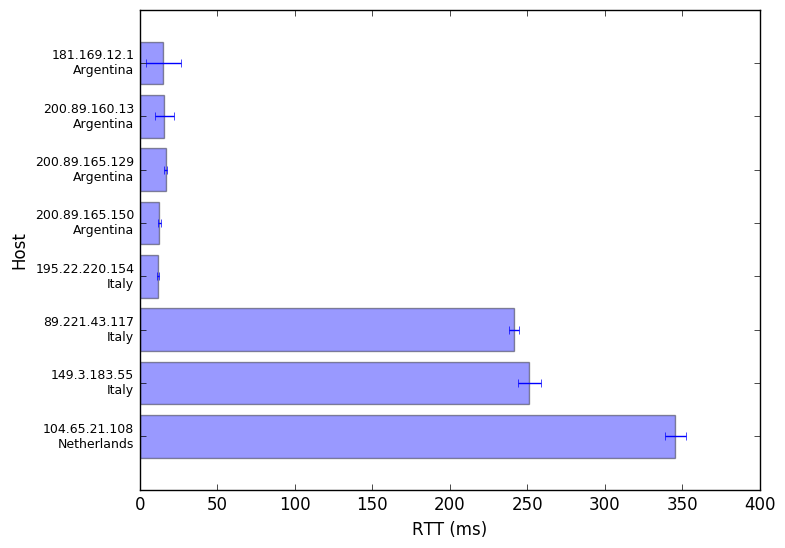
\includegraphics[width=\textwidth,keepaspectratio]{images/mit.png}
\end{figure}

Curiosamente, al final el request termino en Holanda en nodo de Akamai y no en Estados Unidos. Haciendo un Whois al URL confirmamos que esto es correcto.

\begin{table}[H]
\caption{Detección de enlaces intercontinentales: mit.edu}
\centering
\begin{tabular}{@{}llllll@{}}
\toprule
Id & From & To & Avg. RTT & Simbala & GeoIP\\ \midrule
1 & \parbox[t][1.3cm]{5cm}{181.169.12.1 \\ Argentina, SA \\ fibertel.com.ar} & \parbox[t][1.3cm]{5cm}{200.89.160.17 \\ Argentina, SA \\ fibertel.com.ar} & 7.4494 ms & no & no\\ \bottomrule
2 & \parbox[t][1.3cm]{5cm}{195.22.220.152 \\ Italy, EU \\ bai.seabone.net} & \parbox[t][1.3cm]{5cm}{195.22.209.63 \\ Italy, EU \\ lon.seabone.net} & 232.3924 ms & yes & no\\ \bottomrule
3 & \parbox[t][1.3cm]{5cm}{149.3.183.1 \\ Italy, EU \\ } & \parbox[t][1.3cm]{5cm}{104.65.21.108 \\ Netherlands, EU \\ static.akamaitechnologies.com} & 12.4086 ms & no & no\\ \bottomrule

\end{tabular}
\end{table}

Como podemos observar, el método de Simbala detecto un enlace intercontinental. La base de datos de GeoIP ubico al IP source en Italia. Sin embargo el hostname da evidencia a favor de que el mismo en realidad se encuentra en Buenos Aires. Los sitios de geolocalizacion online confirman esto. Es decir, el enlace 2 efectivamente es intercontinental.

\subsubsection{ox.ac.uk}

\begin{table}[H]
\caption{traceroute: ox.ac.uk (oxford)}
\centering
\begin{tabular}{@{}l|llll@{}}
\toprule
Hop & Avg. RTT & IP Address & Host name & Location\\ \midrule
1 & 12.1034 ms & 181.169.12.1 & 1-12-169-181.fibertel.com.ar & Argentina\\
2 &  * * * * * &  &  &  \\
3 &  * * * * * &  &  &  \\
4 &  * * * * * &  &  &  \\
5 & 13.949 ms & 200.89.160.13 & 13-160-89-200.fibertel.com.ar & Argentina\\
6 & 13.857 ms & 200.89.165.250 & 250-165-89-200.fibertel.com.ar & Argentina\\
7 &  * * * &  &  &  \\
7 & 10.7125 ms & 190.216.88.33 &  & Argentina\\
8 & 142.5634 ms & 67.17.99.233 & ae0-300G.ar5.MIA1.gblx.net & United States\\
9 &  * * * * * &  &  &  \\
10 &  * * * * &  &  &  \\
10 & 292.234 ms & 4.69.143.190 & ae-1-3104.ear2.London2.Level3.net & United States\\
11 & 227.1146 ms & 212.187.139.166 & unknown.Level3.net & United Kingdom\\
12 & 227.4534 ms & 146.97.33.2 & ae29.londpg-sbr2.ja.net & United Kingdom\\
13 & 238.4376 ms & 146.97.37.194 & ae19.readdy-rbr1.ja.net & United Kingdom\\
14 & 227.6364 ms & 193.63.108.94 & ae2.oxfoii-rbr1.ja.net & United Kingdom\\
15 & 226.9026 ms & 193.63.108.98 & ae3.oxforq-rbr1.ja.net & United Kingdom\\
16 & 229.074 ms & 193.63.109.90 & oxford-university.ja.net & United Kingdom\\
17 &  * * * * * &  &  &  \\
18 &  * * * * * &  &  &  \\
19 & 242.347 ms & 192.76.32.62 & boucs-lompi1.sdc.ox.ac.uk & United Kingdom\\
20 & 235.7944 ms & 129.67.242.155 & aurochs-web-155.nsms.ox.ac.uk & United Kingdom\\

\end{tabular}
\label{oxford}
\end{table}

Aquí podemos identificar claramente enlaces transatlánticos a partir del host name y la ubicación. Level3 es una empresa conocida proveedora de enlaces. Un dato de color, sus acciones cotizan en Nasdaq.

\begin{figure}[H]
\caption{RTTs de los hosts hasta ox.ac.uk}
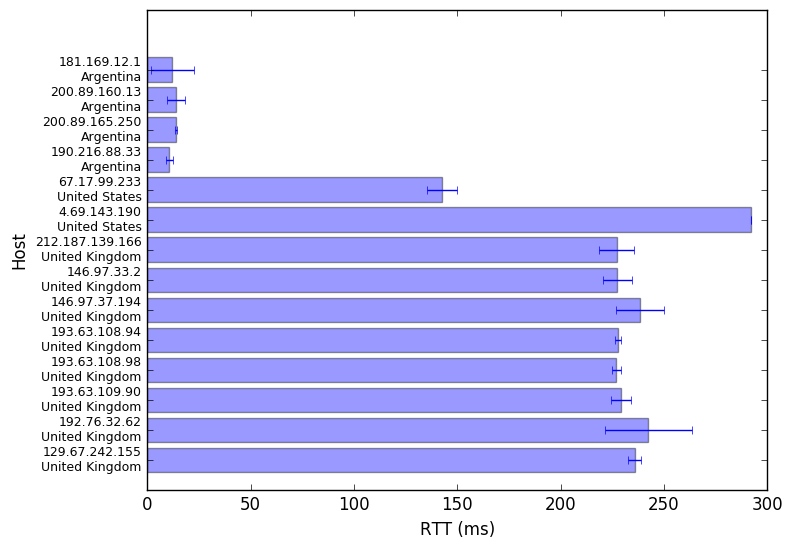
\includegraphics[width=\textwidth,keepaspectratio]{images/oxford.png}
\end{figure}

\begin{table}[H]
\caption{Detección de enlaces intercontinentales: ox.ac.uk}
\centering
\begin{tabular}{@{}llllll@{}}
\toprule
Id & From & To & Avg. RTT & Simbala & GeoIP\\ \midrule
1 & \parbox[t][1.3cm]{5cm}{181.169.12.1 \\ Argentina, SA \\ fibertel.com.ar} & \parbox[t][1.3cm]{5cm}{200.89.160.13 \\ Argentina, SA \\ fibertel.com.ar} & 1.8456 ms & no & no\\ \bottomrule
2 & \parbox[t][1.3cm]{5cm}{200.89.160.13 \\ Argentina, SA \\ fibertel.com.ar} & \parbox[t][1.3cm]{5cm}{200.89.165.250 \\ Argentina, SA \\ fibertel.com.ar} & - & no & no\\ \bottomrule
3 & \parbox[t][1.3cm]{5cm}{200.89.165.250 \\ Argentina, SA \\ fibertel.com.ar} & \parbox[t][1.3cm]{5cm}{190.216.88.33 \\ Argentina, SA \\ } & - & no & no\\ \bottomrule
4 & \parbox[t][1.3cm]{5cm}{190.216.88.33 \\ Argentina, SA \\ } & \parbox[t][1.3cm]{5cm}{67.17.99.233 \\ United States, NA \\ MIA1.gblx.net} & 131.8509 ms & yes & yes\\ \bottomrule
5 & \parbox[t][1.3cm]{5cm}{67.17.99.233 \\ United States, NA \\ MIA1.gblx.net} & \parbox[t][1.3cm]{5cm}{4.69.143.190 \\ United States, NA \\ London2.Level3.net} & 149.6706 ms & yes & no\\ \bottomrule
6 & \parbox[t][1.3cm]{5cm}{4.69.143.190 \\ United States, NA \\ London2.Level3.net} & \parbox[t][1.3cm]{5cm}{212.187.139.166 \\ United Kingdom, EU \\ unknown.Level3.net} & -  & no & yes\\ \bottomrule
7 & \parbox[t][1.3cm]{5cm}{212.187.139.166 \\ United Kingdom, EU \\ unknown.Level3.net} & \parbox[t][1.3cm]{5cm}{146.97.33.2 \\ United Kingdom, EU \\ londpg-sbr2.ja.net} & 0.3388 ms & no & no\\ \bottomrule
8 & \parbox[t][1.3cm]{5cm}{146.97.33.2 \\ United Kingdom, EU \\ londpg-sbr2.ja.net} & \parbox[t][1.3cm]{5cm}{146.97.37.194 \\ United Kingdom, EU \\ readdy-rbr1.ja.net} & 10.9842 ms & no & no\\ \bottomrule
9 & \parbox[t][1.3cm]{5cm}{146.97.37.194 \\ United Kingdom, EU \\ readdy-rbr1.ja.net} & \parbox[t][1.3cm]{5cm}{193.63.108.94 \\ United Kingdom, EU \\ oxfoii-rbr1.ja.net} & - & no & no\\ \bottomrule
10 & \parbox[t][1.3cm]{5cm}{193.63.108.94 \\ United Kingdom, EU \\ oxfoii-rbr1.ja.net} & \parbox[t][1.3cm]{5cm}{193.63.108.98 \\ United Kingdom, EU \\ oxforq-rbr1.ja.net} & - & no & no\\ \bottomrule
11 & \parbox[t][1.3cm]{5cm}{193.63.108.98 \\ United Kingdom, EU \\ oxforq-rbr1.ja.net} & \parbox[t][1.3cm]{5cm}{193.63.109.90 \\ United Kingdom, EU \\ oxford-university.ja.net} & 2.1714 ms & no & no\\ \bottomrule
12 & \parbox[t][1.3cm]{5cm}{193.63.109.90 \\ United Kingdom, EU \\ oxford-university.ja.net} & \parbox[t][1.3cm]{5cm}{192.76.32.62 \\ United Kingdom, EU \\ ox.ac.uk} & 13.273 ms & no & no\\ \bottomrule
13 & \parbox[t][1.3cm]{5cm}{192.76.32.62 \\ United Kingdom, EU \\ ox.ac.uk} & \parbox[t][1.3cm]{5cm}{129.67.242.155 \\ United Kingdom, EU \\ ox.ac.uk} & -  & no & no\\ \bottomrule

\end{tabular}
\end{table}

El enlace numero 4 claramente es intercontinental. Nuevamente nos encontramos con un error de la base de datos de GeoIP en el enlace numero 5, que también es intercontinental aunque el nodo de destino esta etiquetado incorrectamente. En el enlace numero 6 no tenemos un RTT pero GeoIP lo clasifica correctamente como intercontinental.

\subsubsection{u-tokyo.ac.jp}

\begin{table}[H]
\caption{traceroute: u-tokyo.ac.jp}
\centering
\begin{tabular}{@{}l|llll@{}}
\toprule
Hop & Avg. RTT & IP Address & Host name & Location\\ \midrule
1 & 10.9274 ms & 181.169.12.1 & 1-12-169-181.fibertel.com.ar & Argentina\\
2 &  * * * * * &  &  &  \\
3 &  * * * * * &  &  &  \\
4 &  * * * * * &  &  &  \\
5 & 14.2606 ms & 200.89.160.21 & 21-160-89-200.fibertel.com.ar & Argentina\\
6 & 12.1018 ms & 200.89.165.222 & 222-165-89-200.fibertel.com.ar & Argentina\\
7 & 12.8424 ms & 195.22.220.102 & xe-1-0-3.baires5.bai.seabone.net & Italy\\
8 & 40.0902 ms & 195.22.219.17 & ae7.sanpaolo8.spa.seabone.net & Italy\\
9 & 39.1184 ms & 195.22.219.17 & ae7.sanpaolo8.spa.seabone.net & Italy\\
10 & 41.755 ms & 149.3.181.65 &  & Italy\\
11 & 163.8182 ms & 129.250.2.227 & ae-4.r24.nycmny01.us.bb.gin.ntt.net & United States\\
12 & 226.2194 ms & 129.250.4.13 & ae-2.r20.sttlwa01.us.bb.gin.ntt.net & United States\\
13 & 237.003 ms & 129.250.2.54 & ae-0.r21.sttlwa01.us.bb.gin.ntt.net & United States\\
14 & 387.993 ms & 129.250.3.86 & ae-2.r20.osakjp02.jp.bb.gin.ntt.net & United States\\
15 & 403.096 ms & 129.250.6.188 & ae-4.r22.osakjp02.jp.bb.gin.ntt.net & United States\\
16 & 382.5294 ms & 129.250.2.255 & ae-1.r01.osakjp02.jp.bb.gin.ntt.net & United States\\
17 & 393.0274 ms & 61.200.80.218 & xe-0-4-0-7.r01.osakjp02.jp.ce.gin.ntt.net & Japan\\
18 & 392.6634 ms & 158.205.192.173 & ae0.ostcr01.idc.jp & Japan\\
19 & 402.713 ms & 158.205.192.86 &  & Japan\\
20 & 395.828 ms & 158.205.121.250 & po2.l321.fk1.eg.idc.jp & Japan\\
21 & 399.557 ms & 154.34.240.254 &  & Japan\\
22 & 388.1666 ms & 210.152.135.178 &  & Japan\\

 \bottomrule
\end{tabular}
\label{tokyo}
\end{table}

\vspace{10px}

Como era de esperar, este termino siendo el traceroute mas largo, pasando por un camino sumamente raro. De Argentina a Italia, luego a EE.UU. y finalmente a Japón. Sin embargo, si vemos esto desde un punto de vista económico tiene sentido. El trafico desde América Latina a Japon no debe ser muy alto, por lo que no se justifican los altos costos de hacer un enlace mas directo.

Encontramos nuevamente los enlaces transatlánticos de Sparkle. Entrando a ntt.net nos encontramos con:

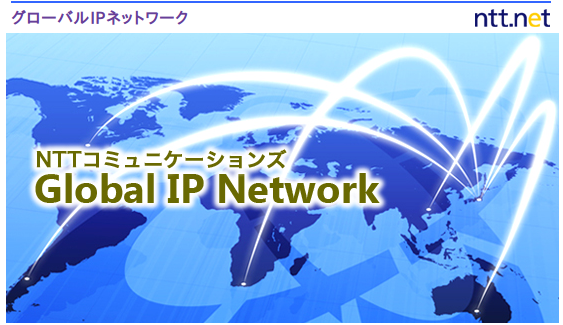
\includegraphics[width=\textwidth,keepaspectratio]{images/ntt}

Esto nos hace inferir que es una empresa Japonesa de telecomunicaciones.

\begin{table}[H]
\caption{Detección de enlaces intercontinentales: u-tokyo.ac.jp}
\centering
\begin{tabular}{@{}llllll@{}}
\toprule
Id & From & To & Avg. RTT & Simbala & GeoIP\\ \midrule
1 & \parbox[t][1.3cm]{5cm}{181.169.12.1 \\ Argentina, SA \\ fibertel.com.ar} & \parbox[t][1.3cm]{5cm}{200.89.160.21 \\ Argentina, SA \\ fibertel.com.ar} & 3.3332 ms & no & no\\ \bottomrule
2 & \parbox[t][1.3cm]{5cm}{200.89.160.21 \\ Argentina, SA \\ fibertel.com.ar} & \parbox[t][1.3cm]{5cm}{200.89.165.222 \\ Argentina, SA \\ fibertel.com.ar} & -  & no & no\\ \bottomrule
3 & \parbox[t][1.3cm]{5cm}{200.89.165.222 \\ Argentina, SA \\ fibertel.com.ar} & \parbox[t][1.3cm]{5cm}{195.22.220.102 \\ Italy, EU \\ bai.seabone.net} & 0.7406 ms & no & yes\\ \bottomrule
4 & \parbox[t][1.3cm]{5cm}{195.22.220.102 \\ Italy, EU \\ bai.seabone.net} & \parbox[t][1.3cm]{5cm}{195.22.219.17 \\ Italy, EU \\ spa.seabone.net} & 27.2478 ms & yes & no\\ \bottomrule
5 & \parbox[t][1.3cm]{5cm}{195.22.219.17 \\ Italy, EU \\ spa.seabone.net} & \parbox[t][1.3cm]{5cm}{195.22.219.17 \\ Italy, EU \\ spa.seabone.net} & -  & no & no\\ \bottomrule
6 & \parbox[t][1.3cm]{5cm}{195.22.219.17 \\ Italy, EU \\ spa.seabone.net} & \parbox[t][1.3cm]{5cm}{149.3.181.65 \\ Italy, EU \\ } & 2.6366 ms & no & no\\ \bottomrule
7 & \parbox[t][1.3cm]{5cm}{149.3.181.65 \\ Italy, EU \\ } & \parbox[t][1.3cm]{5cm}{129.250.2.227 \\ United States, NA \\ gin.ntt.net} & 122.0632 ms & yes & yes\\ \bottomrule
8 & \parbox[t][1.3cm]{5cm}{129.250.2.227 \\ United States, NA \\ gin.ntt.net} & \parbox[t][1.3cm]{5cm}{129.250.4.13 \\ United States, NA \\ gin.ntt.net} & 62.4012 ms & yes & no\\ \bottomrule
9 & \parbox[t][1.3cm]{5cm}{129.250.4.13 \\ United States, NA \\ gin.ntt.net} & \parbox[t][1.3cm]{5cm}{129.250.2.54 \\ United States, NA \\ gin.ntt.net} & 10.7836 ms & no & no\\ \bottomrule
10 & \parbox[t][1.3cm]{5cm}{129.250.2.54 \\ United States, NA \\ gin.ntt.net} & \parbox[t][1.3cm]{5cm}{129.250.3.86 \\ United States, NA \\ gin.ntt.net} & 150.99 ms & yes & no\\ \bottomrule
11 & \parbox[t][1.3cm]{5cm}{129.250.3.86 \\ United States, NA \\ gin.ntt.net} & \parbox[t][1.3cm]{5cm}{129.250.6.188 \\ United States, NA \\ gin.ntt.net} & 15.103 ms & no & no\\ \bottomrule
12 & \parbox[t][1.3cm]{5cm}{129.250.6.188 \\ United States, NA \\ gin.ntt.net} & \parbox[t][1.3cm]{5cm}{129.250.2.255 \\ United States, NA \\ gin.ntt.net} & -  & no & no\\ \bottomrule
13 & \parbox[t][1.3cm]{5cm}{129.250.2.255 \\ United States, NA \\ gin.ntt.net} & \parbox[t][1.3cm]{5cm}{61.200.80.218 \\ Japan, AS \\ gin.ntt.net} & 10.498 ms & no & yes\\ \bottomrule
14 & \parbox[t][1.3cm]{5cm}{61.200.80.218 \\ Japan, AS \\ gin.ntt.net} & \parbox[t][1.3cm]{5cm}{158.205.192.173 \\ Japan, AS \\ ostcr01.idc.jp} & -  & no & no\\ \bottomrule
15 & \parbox[t][1.3cm]{5cm}{158.205.192.173 \\ Japan, AS \\ ostcr01.idc.jp} & \parbox[t][1.3cm]{5cm}{158.205.192.86 \\ Japan, AS \\ } & 10.0496 ms & no & no\\ \bottomrule
16 & \parbox[t][1.3cm]{5cm}{158.205.192.86 \\ Japan, AS \\ } & \parbox[t][1.3cm]{5cm}{158.205.121.250 \\ Japan, AS \\ eg.idc.jp} & -  & no & no\\ \bottomrule
17 & \parbox[t][1.3cm]{5cm}{158.205.121.250 \\ Japan, AS \\ eg.idc.jp} & \parbox[t][1.3cm]{5cm}{154.34.240.254 \\ Japan, AS \\ } & 3.729 ms & no & no\\ \bottomrule
18 & \parbox[t][1.3cm]{5cm}{154.34.240.254 \\ Japan, AS \\ } & \parbox[t][1.3cm]{5cm}{210.152.135.178 \\ Japan, AS \\ } & - & no & no\\ \bottomrule


\end{tabular}
\end{table}

El enlace numero 4 es el primer enlace intercontinental entre Argentina e Italia. En este caso el método de Simbala si logra identificarlo, mientras que GeoIP tiene datos incorrectos. El próximo enlace es el numero 7 entre Italia y Estados Unidos. Ambos métodos logran identificarlos. Luego Simbala no clasifica bien los enlaces numero 8 y 10. Solo GeoIP logra identificar satisfactoriamente el enlace numero 13.

\subsection{Caching}

Este experimento fue una casualidad. Al hacer dos requests a google.com, notamos que mientras una traza hacia un salto intercontinental, la otra no. Allí nos dimos cuenta que en realidad lo que sucedía era que Fibertel hace caching, lo que baja el RTT en un tercio. Suponemos que esto debe ser sumamente útil para proveer a usuarios que utilizan streaming y P2P.

\begin{table}[H]
\caption{traceroute: google.com sin caching}
\centering
\begin{tabular}{@{}l|llll@{}}
\toprule
Hop & Avg. RTT & IP Address & Host name & Location\\ \midrule
1 & 10.6688 ms & 181.169.12.1 & 1-12-169-181.fibertel.com.ar & AR, SA\\
2 &  * * * * * &  &  &  \\
3 &  * * * * * &  &  &  \\
4 &  * * * * * &  &  &  \\
5 & 20.2096 ms & 200.89.160.21 & 21-160-89-200.fibertel.com.ar & AR, SA\\
6 & 14.3278 ms & 200.89.165.129 & 129-165-89-200.fibertel.com.ar & AR, SA\\
7 & 12.5566 ms & 200.89.165.150 & 150-165-89-200.fibertel.com.ar & AR, SA\\
8 &  * * * * * &  &  &  \\
9 & 10.9052 ms & 209.85.251.86 & 209.85.251.86 & US, NA\\
10 & 40.759 ms & 209.85.252.42 & 209.85.252.42 & US, NA\\
11 & 38.5816 ms & 216.239.58.221 & 216.239.58.221 & US, NA\\
12 & 38.1802 ms & 216.58.202.4 & gru06s26-in-f4.1e100.net & US, NA\\ \bottomrule
\end{tabular}
\label{google}
\end{table}


\begin{table}[H]
\caption{traceroute: google.com con caching}
\centering
\begin{tabular}{@{}l|llll@{}}
\toprule
Hop & Avg. RTT & IP Address & Host name & Location\\ \midrule
1 & 11.1854 ms & 181.169.12.1 & 1-12-169-181.fibertel.com.ar & AR, SA\\
2 &  * * * * * &  &  &  \\
3 &  * * * * * &  &  &  \\
4 &  * * * * * &  &  &  \\
5 & 21.9184 ms & 200.89.165.33 & 33-165-89-200.fibertel.com.ar & AR, SA\\
6 & 15.066 ms & 200.89.164.26 & 26-164-89-200.fibertel.com.ar & AR, SA\\
7 &  * * * * * &  &  &  \\
8 & 11.6574 ms & 181.30.241.187 & 187-241-30-181.fibertel.com.ar & AR, SA\\ \bottomrule
\end{tabular}
\label{googlecache}
\end{table}